\documentclass[../Bachelorarbeit.tex]{subfiles}

\begin{document}
\label{sec:LHC}
\section{Large Hadron Collider}
CERN may be the most famous scientific institution in the world. One reason for this fame is the Large Hadron Collider (\acrshort{lhc})\cite{Evans.2008} build in 2008. The \acrshort{lhc} is the largest circular collider in the world,
famous for the first discovery of the Higgs-Boson. The two-ring-superconducting- hadron accelerator and collider are build in a 26.7 km tunnel beneath the France–Switzerland border.
This technological marble is only possible thanks to thousands of engineers, computer scientists and physicists around the world.
Four large detectors ALICE, ATLAS, CMS and \acrshort{lhc} and other smaller experiments are connected to the \acrshort{lhc}.
The \acrshort{lhc} aims for a collision energy of 14 TeV and as of now Run-II achieved 13 TeV by accelerating particle beams up to 6.5 TeV.\\\\
The number of events per second N is given by:
\begin{equation}
    \frac{dN}{dt} = L \sigma
\end{equation}

$\sigma$ is the cross-section of particles and L the luminosity defined as:
\footnote{Equations taken from \cite{Evans.2008}}

\begin{equation}
    L= \frac{N_{b}^{2} n_{b} f \gamma}{5 \pi \epsilon_{n} \beta^{*}} F \qquad \textnormal{ with } \qquad  F=\left( 1 + \left( \frac{\theta_{c} \sigma_{z}}{2 \sigma^{*}}\right)^{2} \right)^{-\frac{1}{2}}
\end{equation}

\begin{description}
    \item[$N_{b}$] number of particles per bunch
    \item[$n_{b}$]  number of bunches
    \item[$\epsilon_{n}$]  normalized transverse beam emittance
    \item[$\beta^{*}$] beta function at collision point
    \item[$F$] luminosity correction in the interaction point based on the crossing angle
\end{description}
With the start of Run-3 on April 22, 2022 a collision energy of 13.6 TeV is expected.
\begin{figure}
    \centering
    \includegraphics[width=0.8\textwidth]{images/CCC-v2022.jpg}
    \caption{Schematic view of the \acrshort{lhc} with all experiments \cite{CERN.01.05.2022}}
    \label{fig:LHC_schematic}
\end{figure}

\section{ATLAS detector}
ATLAS\footnote{\textbf{A} \textbf{T}oroidal \acrshort{lhc} \textbf{A}pparatu\textbf{S}} the largest general-purpose detector is a part of the \acrshort{lhc} experiments with more than 5500 scientists working on
ATLAS experiments worldwide. The main goal is precision measurements but also Higgs search, extra dimension, dark matter and a wide variety of physics research is conducted.
A short overview of the ATLAS detectors structure is shown here in figure \ref{fig:ALTAS_detector}, but a detailed version can be read here \cite{Evans.2008}.
\\\\
\textbf{Magnet System}\\
The magnet system creates the magnetic field that bends the trajectory of the incoming particles in order to measure the momentum of said particles.
For this purpose two superconducting toroide magnets create a magnetic field $B=2$ T. The momentum can be calculated from the curvature $r$ due to the Lorenz force.
\begin{equation}
    r=\frac{p}{q B}
\end{equation}
where $p=\gamma m v$ is the relativistic momentum and $q$ the charge of the particle. High momentum-particles result in small curvature while low-momentum particles show a greater curvature.
\\\\
\textbf{Inner Detector}\\
The inner detector consists of three subdetectors. The ATLAS-Pixel detector is the innermost part surrounded by the semiconductor tracker(SCT) providing additional data for the curvature calculation.
The outermost layer is the transition radiation tracker (TRT). Transition radiation is used to differentiate between fermions and hadrons.
\\\\
\textbf{Calorimeters}
The electromagnetic calorimeter and the Hadron calorimeter make up the calorimeter system. Particles that interact via electromagnetic force are measured in
the electromagnetic calorimeter. Electrons or photons create particle showers in the electromagnetic calorimeter and no showers in the hadronic calorimeter while hadrons show traces in both and showers mostly in the hadronic calorimeter(as shown in \ref{fig:calorimeter}).
This happens because hadrons have a higher mass and the cross-section ins inverse proportional to the mass of the particle.
\\\\
\textbf{Myon Spectrometer}
Two different myon detectors are used for ATLAS experiments. First the precision chambers for spatial resolution measurements while the second detector is mainly used as a trigger. Interesting myon events can be analysed
independent of other events as myon have heavy mass and don't decay though strong interactions, therefore only traces are visible in the first two detectors.

\begin{figure}[h]
    \begin{subfigure}{0.59\textwidth}
        \centering
        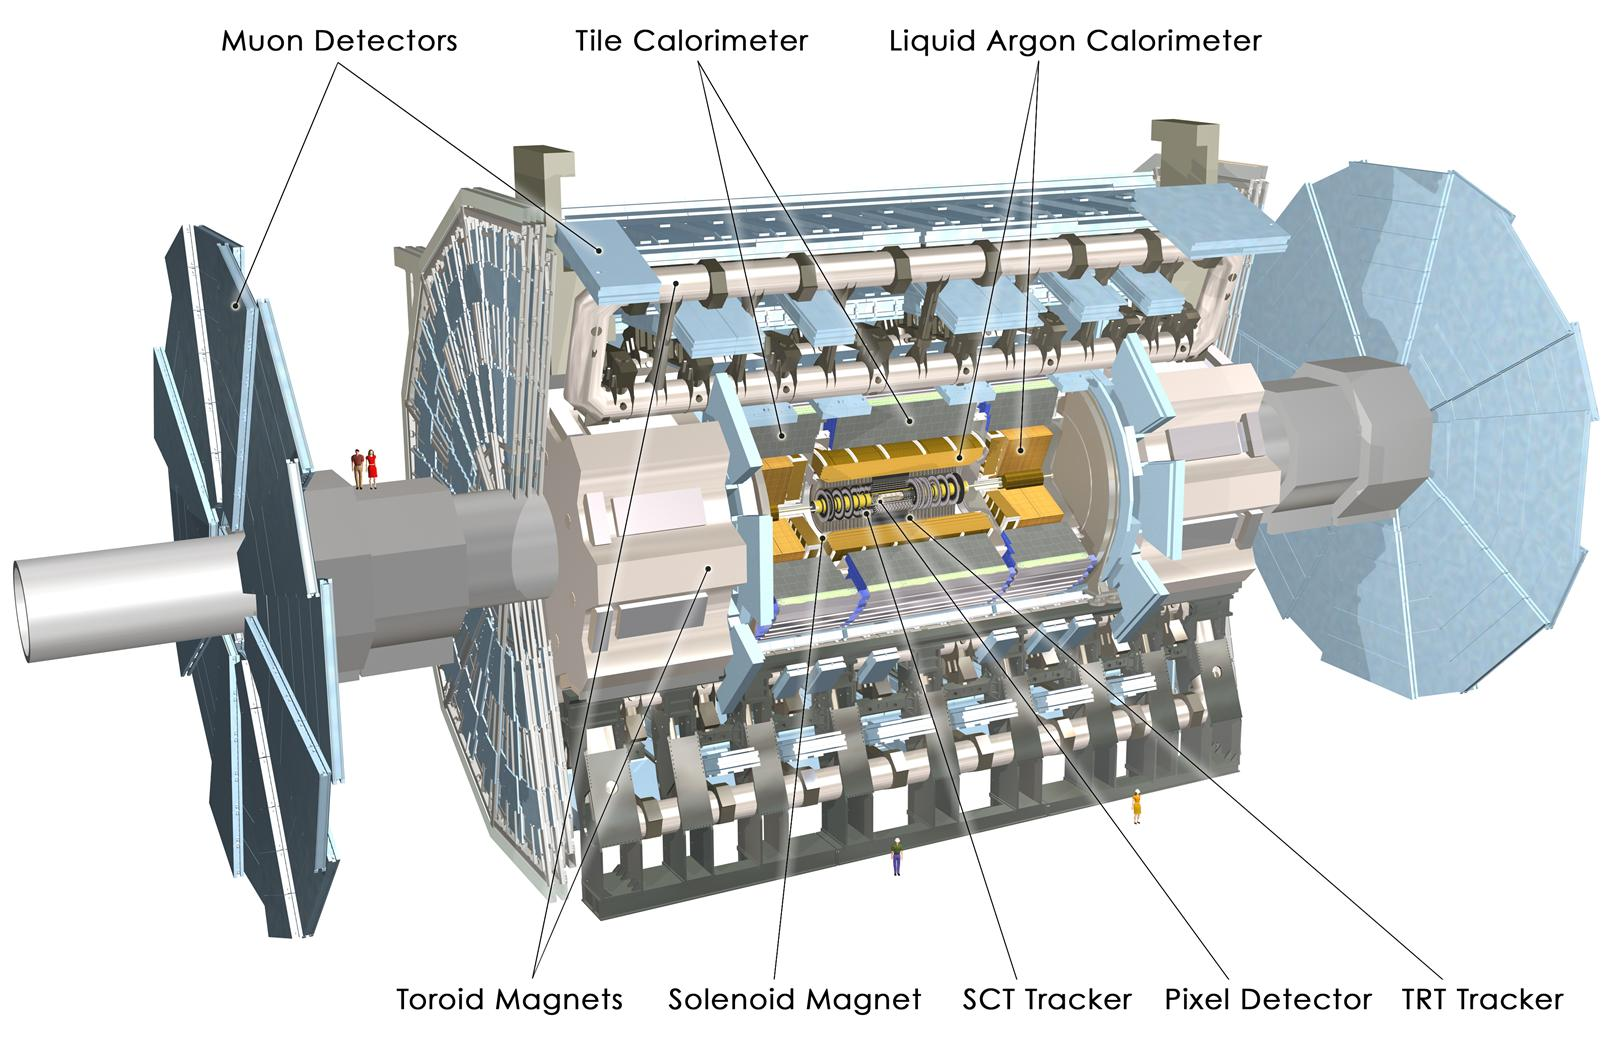
\includegraphics[width=\textwidth]{images/0803012_05-A4-at-144-dpi.jpg}
        \caption{}
        \label{fig:ALTAS_detector}
    \end{subfigure}
    \begin{subfigure}{0.40\textwidth}
        \centering
        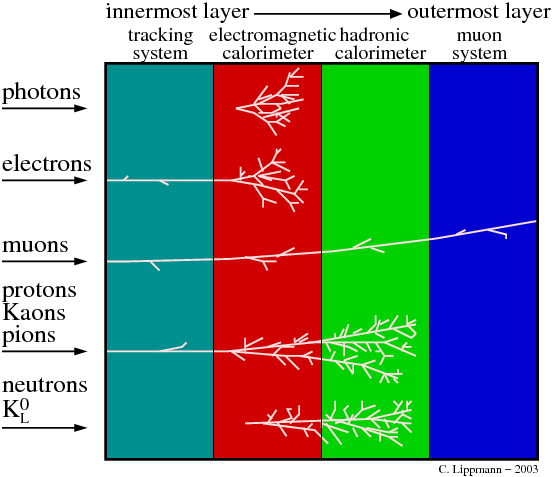
\includegraphics[width=\textwidth]{images/experiment_atlas.png}
        \caption{}
        \label{fig:calorimeter}
    \end{subfigure}
    \caption{\textbf{a)}3D of the ATLAS detectors with major components \cite{JoaoPequenao.27.03.2008} \textbf{b)} Schematic of particle showers and traces inside the ATLAS detector \cite{Lippmann.2012}}
\end{figure}
\end{document}
